\documentclass[11pt]{asaproc}

\usepackage{graphicx}
\usepackage{natbib}
\usepackage[hyphens]{url}
\usepackage{color}
\usepackage{times}
\usepackage{verbatim}
%\usepackage{enumitem}
\usepackage[hidelinks,breaklinks=true]{hyperref}

\renewcommand\labelenumi{(\roman{enumi})}
\renewcommand\theenumi\labelenumi

\title{Eye-Tracking in Practice: A First Analysis of a Study on Human Postures}

\author{J\"{u}rgen Symanzik \thanks{Department of Mathematics and Statistics, Utah State University, Logan, UT 84322--3900, USA. 
E-mail: \url{symanzik@math.usu.edu}}
 \and Chunyang Li \thanks{Department of Mathematics and Statistics, Utah State University, Logan, UT 84322--3900, USA. 
E-mail: \url{lichunyang1990@hotmail.com}}
 \and Boyu Zhang \thanks{Department of Computer Science, Utah State University, Logan, UT 84322--3900, USA. 
E-mail: \url{boyu.zhang@aggiemail.usu.edu}}
 \and Breanna Studenka \thanks{Department of Kinesiology and Health Science, Utah State University, Logan, UT 84322--3900, USA. 
E-mail: \url{Breanna.studenka@usu.edu}}
 \and Eric McKinney \thanks{Department of Mathematics and Statistics, Utah State University, Logan, UT 84322--3900, USA. 
E-mail: \url{ericmckinney77@gmail.com}}
}

\begin{document}

\renewcommand{\topfraction}{1.0}
\renewcommand{\bottomfraction}{1.0}
\renewcommand{\textfraction}{0.0}
\renewcommand{\floatpagefraction}{1.0}
\renewcommand{\dbltopfraction}{1.0}


\maketitle

\begin{abstract}In this article, we present our first results of a study that tries to determine where people are looking when ranking the stability of an
actor holding certain postures. A mobile eye-tracker is used to record the original video data of people looking at human
postures. Image processing methods are employed to extract statistical information from the video data. 
The statistical analyses are based on visualization and machine learning approaches.
\end{abstract}

\begin{keywords}Eye-Tracking Data; Image Processing; Visualization; Machine Learning; Software; {\tt EyeTrackR} R Package
\end{keywords}


%%%%%%%%%%%%%%%%%%%%%%%%%
\section{Introduction}
\label{Introduction}
%%%%%%%%%%%%%%%%%%%%%%%%%

An individual's planning and execution of actions is guided by many things, one of which is the anticipated posture at the end-state of an action. Studies on action planning indicate that future postural states can influence the choice of previous postures 
\citep{CR2004,HB2010,RCMV2006}.
%(i.e., Cohen \& Rosenbaum, 2004; Herbort \& Butz, 2010; see Rosenbaum, Cohen, Meulenbroek, \& Vaughan, 2006 for a review). 
For example, when grasping an overturned glass with the intent to pour water into it, the glass is typically grasped with a thumb-down posture so that the glass can be turned upward and the hand can end in a thumb-upward posture. This thumb-upward posture is also rated to be more comfortable than a thumb-down posture, and is therefore one example of the end-state-comfort effect --- the observed phenomenon whereby most actions end with a comfortable posture
\citep{RMBVSJ1990}.
%(Rosenbaum et al., 1990). 

%Cohen, R. G., \& Rosenbaum, D. A. (2004). Where grasps are made reveals how grasps are planned: generation and recall of motor plans. Experimental Brain Research, 157(4), 486-495.
%Herbort, O., \& Butz, M. V. (2010). Planning and control of hand orientation in grasping movements. Experimental Brain Research, 202(4), 867-878.
%Rosenbaum, D. A., Cohen, R. G., Meulenbroek, R. G., \& Vaughan, J. (2006). Plans for grasping objects. Motor control and learning over the lifespan, 9-25.
%Rosenbaum, D. A., Marchak, F., Barnes, H. J., Vaughan, J., Slotta, J. D., \& Jorgensen, M. J. (1990). Constraints for action selection: Overhand versus underhand grips.


The aim of our planned posture study will be to determine whether judgment of other's action capabilities is based on one's own action experiences. We will examine the stability judgments of individuals viewing an actor holding different postures. Two groups of participants will be examined: one group with extensive yoga experience, and one group with minimal experience with actions that require stability (e.g., yoga, gymnastics, ballet dancing, etc.).  We will equip each participant from each group with mobile eye-tracking equipment that will enable us to see what they are looking at as they make stability judgments. We hypothesize that perceptions of others' stability will be influenced by the unique experiences of participants. More specifically, we hypothesize that those with extensive yoga experience will judge an actor to be more stable than those without stability-specific experience.  Furthermore, we hypothesize that the visual information used to judge stability will differ between different groups of individuals with unique action experiences.

This article is structured as follows: In Section~\ref{PostureStudy}, we provide further details on the planned posture study.
In Section~\ref{EDA}, we present preliminary results from two participants that were used to evaluate the final setup
of the full posture study and to assess the functionality of the data recording and data processing.
All of our visualizations and analyses are conducted with the {\tt R} statistical computing platform \citep{RCore2017}.
In Section~\ref{Outlook}, we provide an outlook at the upcoming steps in our full posture study to be conducted in the 2017/2018
academic year.


%%%%%%%%%%%%%%%%%%%%%%%%%
\section{The Posture Study}  
\label{PostureStudy}
%%%%%%%%%%%%%%%%%%%%%%%%%

``Does judging the action capabilities of another person depend on one's own experiences?'' This is the
primary research question for our planned posture study. For many human interactions, 
action anticipation must be present when interacting with others (e.g., 
to avoid collisions, pass something on to someone, etc.). This study is 
motivated by research conducted in the Kinesiology and Health Science Department at Utah State University (USU).

Most literature examining ones perceptions of others' action capabilities involves asking subjects to estimate
the performance of another individual, e.g., ``can Sally reach the block or not?'' \citep{Roc95}. The visual
information used by the participant in making their judgments has been limited to making a participant to
identify in what direction another person might be looking or what they might be looking at \citep{MiZa2006}. We are
unaware of any study looking at the use of eye-tracking to determine what particular visual information about an
actor might be used for judgments about action capabilities. Therefore, no literature exists to describe how
one might
set up and conduct such a human posture study, in particular when incorporating
mobile eye-tracking equipment as a major component of the data recording, data processing, and data analysis.
Numerous preliminary test participants participated to help evaluate and refine the setup of the study.
Data and results from two of these preliminary test participants are presented here. Both 
participated under conditions similar to the final setup of the posture study.

%Rochat, P. (1995). Perceived reachability for self and for others by 3-to 5-year-old children and adults. Journal of Experimental Child Psychology, 59(2), 317-333.
%
%For the other citation:
%Michelon, P., & Zacks, J. M. (2006). Two kinds of visual perspective taking. Attention, Perception, & Psychophysics, 68(2), 327-337.


There will be two groups of participants in the full posture study. In Group~1, there will be 
20 students with minimal experience with actions that require stability (e.g., yoga, gymnastics, ballet dancing, etc.)
from the undergraduate Psychology pool at USU.
In Group~2, there will be 20 students with extensive yoga experience from advanced yoga classes at USU.
We anticipate that 
those with extensive yoga experience will judge an actor to be more stable than those without stability-specific experience.
Moreover, we expect that the visual information used to judge stability will differ between different groups of individuals with 
unique action experiences.

Each of the 40 participants will be shown 22 pictures of a single actor holding a posture.
Twenty-two different postures were derived by systematically developing one posture per axis of rotation and
within each axis of rotation, choosing three postures of increasing difficulty. Three postures were chosen for
sagittal, frontal, and transverse plane rotation, for the combination of sagittal and frontal, sagittal and transverse,
and frontal and transverse, and for the combination of all three planes of rotation.\footnote{The sagittal plane 
divides the human body into left and right halves, the frontal plane into front and back halves,
and the transverse plane into superior and inferior halves.}
Therefore, 21 postures were
developed with the addition of a posture with no rotation. The difficulty of the three postures within each
rotation was arbitrarily determined by the experimenter.
Figure~\ref{SixPostures} shows six of these postures.

All postures were shown to each participant in random order, projected to a wall, one at a time.
Participants were required to judge the stability of each posture (i.e., how long the person could hold the posture).
Possible answers were
$<$ 1sec, 1 -- 10sec, 11sec -- 1min, 1min -- 1hour, and $>$ 1hour.
To avoid ambiguity, the intervals will be slightly modified in the full study:
$\leq$ 1sec,  $>$ 1sec -- 10sec, $>$ 10sec -- 1min, $>$ 1min -- 1hour, and $>$ 1hour.
The participants wore a mobile eye-tracking device from Applied Science Laboratories (ASL), Bedford, MA, for the entire study.
This device uses one camera that continuously records the (changing) scene that is visible for the participant at a frequency of 30 Hz. 
Moreover, the focal point of the right eye is recorded by a second camera of this device and is overlaid as a cross-hair
on each video frame of the recorded scene video. Details on these eye-tracker video recordings and how to extract
the focal point of the eye in each video frame and translate it to the coordinates of a static image of the posture via the
{\tt EyeTrackR} R package can be found in \cite{LS2016ASA,LS2017ASA}.

In practice, a static eye-tracker could have been used as well for this posture study. However, we decided to use the mobile
eye-tracker from ASL for two reasons. First, and most importantly, \cite{Faw2016} reported that the static eye-tracker available
at USU is not very precise for some areas of the computer screen. Thus, fixations from the posture study may not be matched with
the proper body parts. Second, the posture study likely is a precursory step to future, more complex studies
that will require the participants to do some physical movements in combination with recording
the eye movements, e.g., where does a participant look when picking up an item.
Such studies can't be conducted with a static eye-tracker and a mobile eye-tracker must be used instead.  
Therefore, gaining some practical insights from a simpler experiment (such as the posture study) may be valuable
for more complex future studies.


\begin{figure}[t]
\begin{center} 
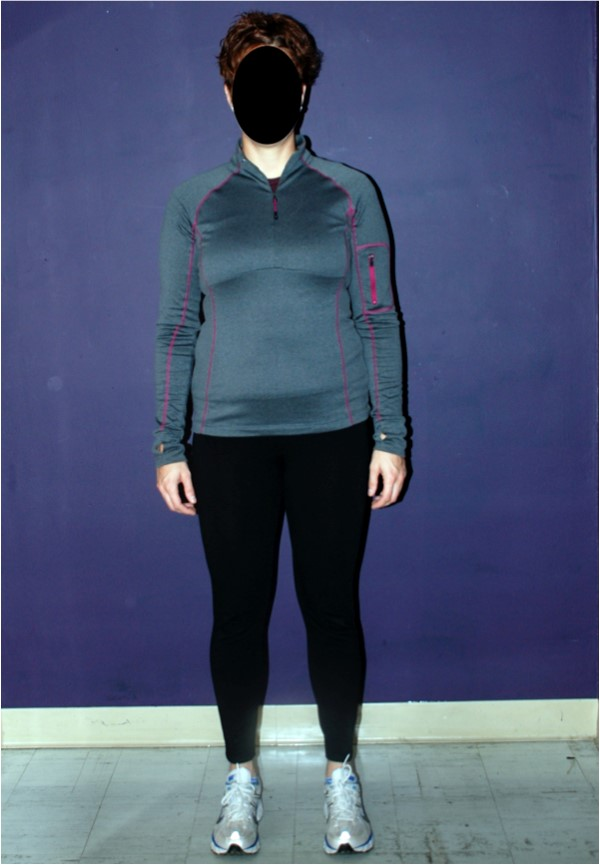
\includegraphics[height=4.3cm,width=4.3cm]{figures/Posture1.jpg} \hspace{1pt}
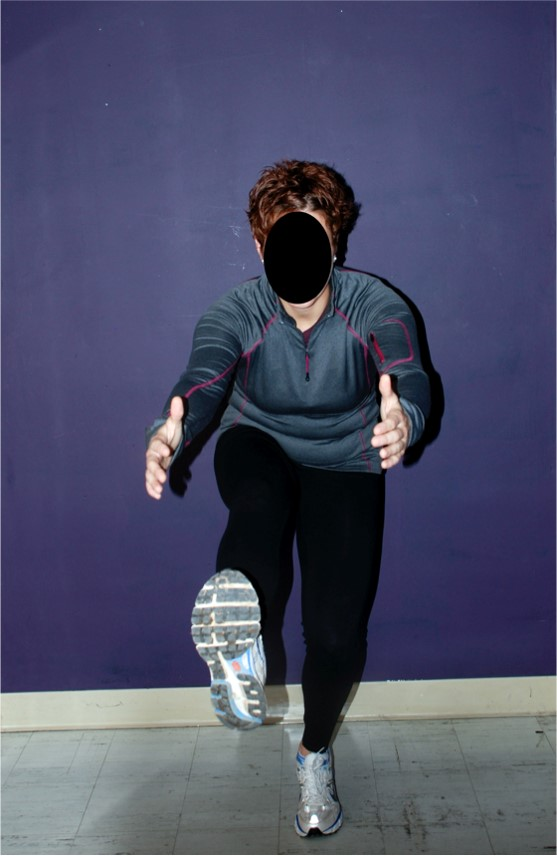
\includegraphics[height=4.3cm,width=4.3cm]{figures/Posture2.jpg} \hspace{1pt}
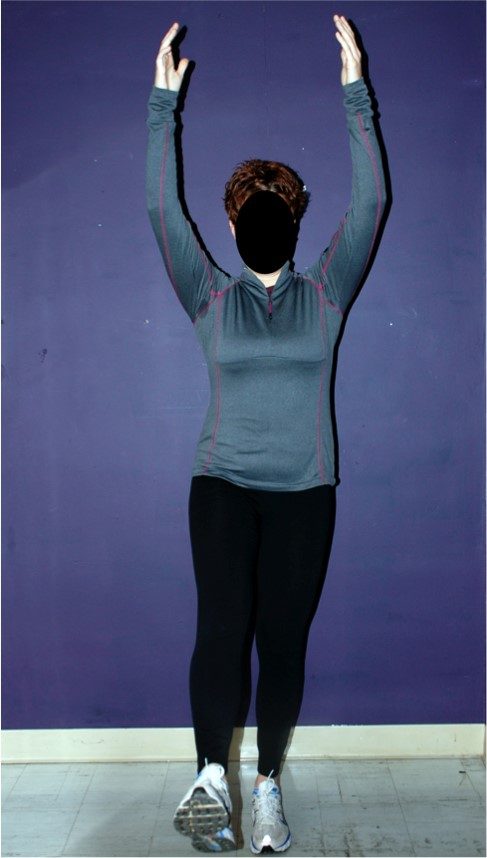
\includegraphics[height=4.3cm,width=4.3cm]{figures/Posture3.jpg} \hspace{1pt} \\
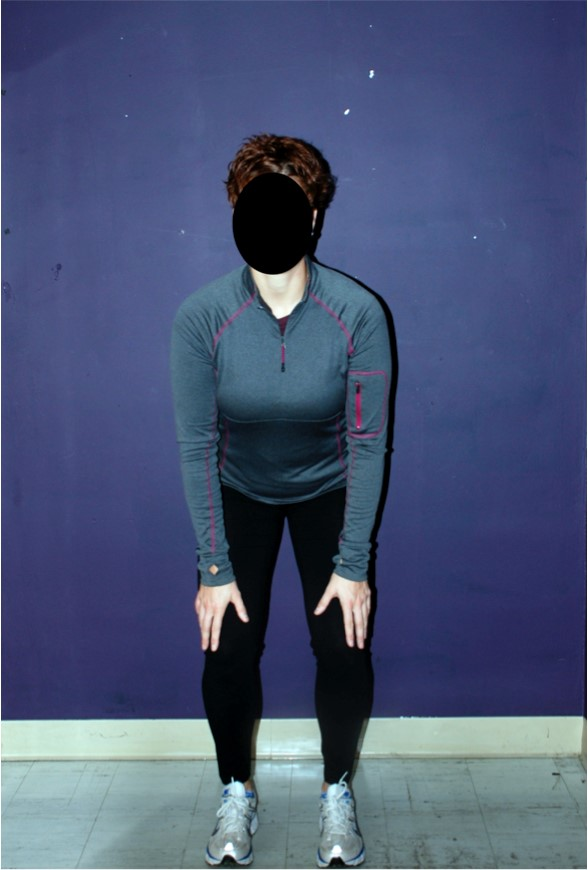
\includegraphics[height=4.3cm,width=4.3cm]{figures/Posture4.jpg} \hspace{1pt}
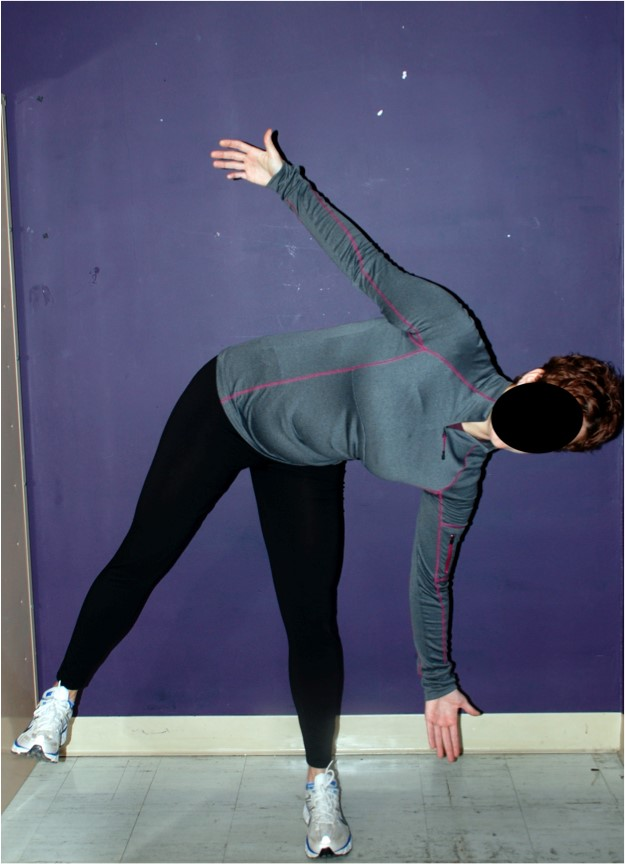
\includegraphics[height=4.3cm,width=4.3cm]{figures/Posture5.jpg} \hspace{1pt}
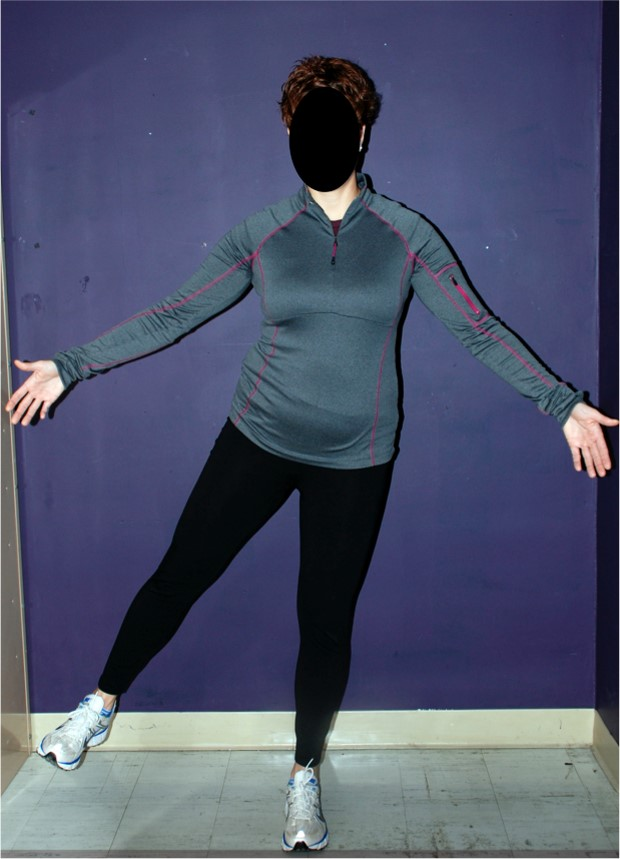
\includegraphics[height=4.3cm,width=4.3cm]{figures/Posture6.jpg} \hspace{1pt}	
\end{center} 
\caption{\label{SixPostures}Postures 1 to 6 (out of 22) used in the study.}
\end{figure}


The data obtained from the eye-tracker allows us to answer several
secondary research questions: At which body parts (such as head, shoulders, hands, elbows, hips, knees, and feet)
do the participants look for each posture? In the context of eye-tracking, these body parts
are the areas of interest (AOIs) in each posture and have to be specified
once for each posture, using the {\tt EyeTrackR} R package.
How long and how often do the participants look at the body parts in each posture?
Are the viewing patterns of the participants associated with the stability assessment?
Methods from machine learning may be used to answer these questions.

The final data collection will consist of 
880 answers to the stability assessment (22 postures $\times$ 20 participants $\times$ 2 groups)
and 40 recordings, i.e., videos, from the eye-tracker (one for each participant).
For the preliminary assessment of two test participants, presented in the next section,
44 answers to the stability assessment (22 postures $\times$ 2 participants)
and two video recordings have been analyzed.


%%%%%%%%%%%%%%%%%%%%%%%%%
\section{Exploratory Data Analysis}  
\label{EDA}
%%%%%%%%%%%%%%%%%%%%%%%%%


For the 40 participants of the full study, we expect to be able to answer questions such as:
\begin{itemize}
\item What are {\bf within groups} similarities / differences (if any) of the viewing patterns for each posture / for all postures?
\item What are {\bf between groups} similarities / differences (if any) of the viewing patterns for each posture / for all postures?
\end{itemize}
For the analysis of the data of the two test participants, we employed various 
exploratory data analysis (EDA) methods commonly used for eye-tracking data.
These methods are (i) eye scatterplots where the participant's focus points are overlaid on the posture;
(ii) attention maps (or hot spot maps) overlaid on the posture; 
(iii) scanpath maps that show the fixations, i.e., the state when the eye remains stable for a (short) period of time, and the saccades,
indicating rapid movement of the eye between two fixations; and
(iv) various types of linked microposter plots, introduced in \cite{LS2016ASA,LS2017ASA}.


\begin{figure}[t]
\begin{center} 
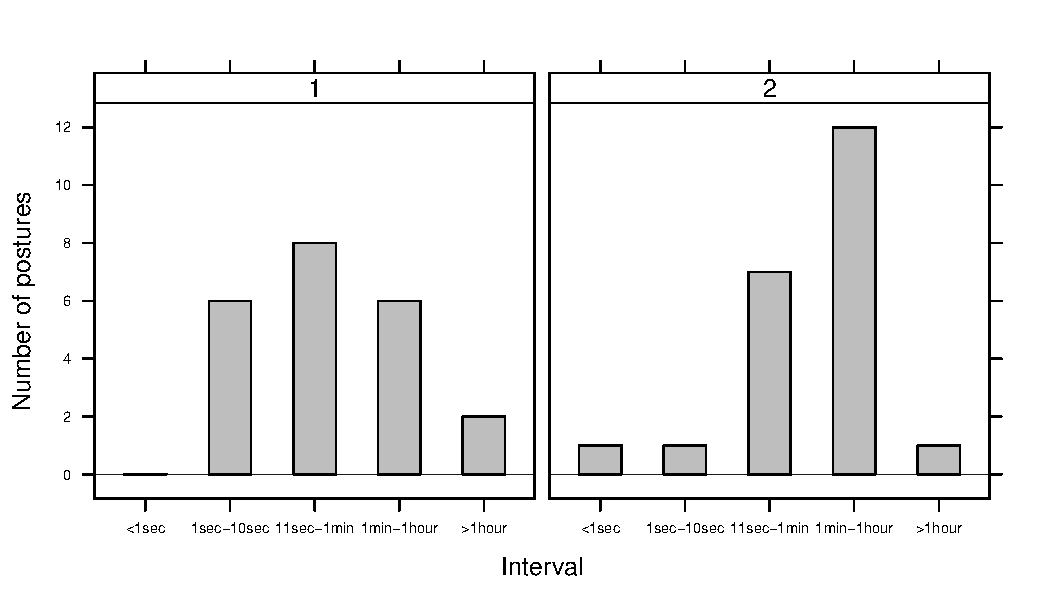
\includegraphics[width=0.99\textwidth]{figures/Participant_1_2_Lengths.pdf}
\end{center} 
\caption{\label{Distributions}Stability assessment distributions for Participant~1 (left) and Participant~2 (right).}
\end{figure}


\begin{figure}[t]
\begin{center} 
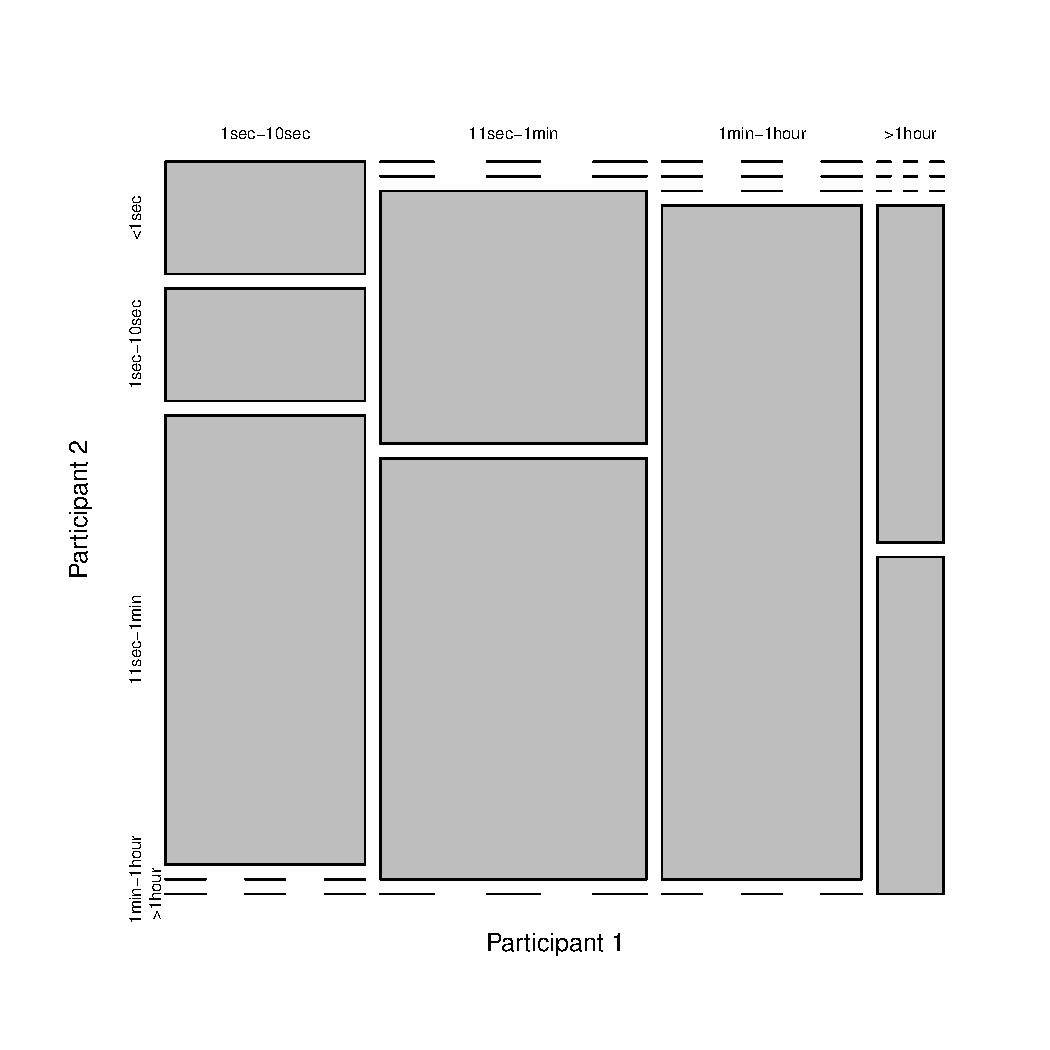
\includegraphics[width=0.9\textwidth]{figures/LengthsAgreements.pdf}
\end{center} ~\\[-2.5cm]
\caption{\label{Comparison}Mosaic plot for the stability assessment comparison of Participant~1 and Participant~2.}
\end{figure}


The stability assessment distributions for the two participants are shown in Figure~\ref{Distributions}.
While the mode for Participant~1 falls into the 11sec -- 1min interval (8 of the 22 postures),
the mode for Participant~2 falls into the 1min -- 1hour interval (12 of the 22 postures).
We expect to see such different distributions for participants from the two groups
in our full study as we hypothesize that 
those with extensive yoga experience (from Group~2) will judge a posture to be more stable than those 
without stability-specific experience.


For the two test participants, there was 
agreement on the stability assessment in 50\% of the postures (11 out of 22)
For the remaining 50\% of the postures, there was a one-level difference,
as shown in Figure~\ref{Comparison}. Most notable, whenever
Participant~1 indicated that a posture could be kept for 1min -- 1hour,
Participant~2 came to the same assessment.
Eventually, in our full study, we expect to see that in a comparison of
participants from Group~1 (on the horizontal axis) and Group~2 (on the vertical axis), more differences will occur
in the triangular area below the diagonal representing identical assessments
than in the triangular area above the diagonal. 
This is because of our hypothesis that
those with extensive yoga experience (from Group~2) will judge a posture to be more stable than those 
without stability-specific experience.


\begin{figure}[t]
\begin{center} 
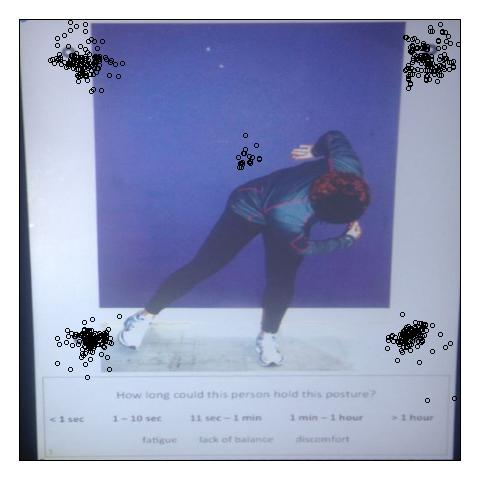
\includegraphics[width=0.49\textwidth]{figures/Kayd_scatterplot_posture0.jpg} \hspace{1pt}
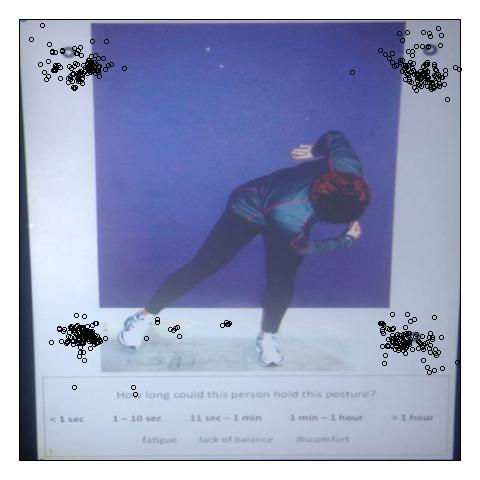
\includegraphics[width=0.49\textwidth]{figures/Kayd_scatterplot_posture23.jpg}
\end{center}
\caption{\label{ScatterplotPrePost}Scatterplot showing the focus points, confirming the proper calibration of the eye-tracking device
at the start of the experiment (left) and end of the experiment (right) for Participant~1.}
\end{figure}


For the two test participants, and also for the participants of the full study, we will use EDA methods
to determine whether the eye-tracking device is properly calibrated before the participant looks
at the 22 postures and remains properly calibrated throughout the entire experiment. This is
done by asking the participants to look at four dots outside the posture area, shown one-by-one
for about two seconds before the 22 postures. 
The posture used for the calibration assessment is an electronically modified version
of one of the actual postures and does not show up in the actual study.
The same four dots also are shown in the same
way after the 22 postures. A simple scatterplot of the focal points, overlaid on this additional posture is then used
to assess the quality of the calibration, here shown for Participant~1 in Figure~\ref{ScatterplotPrePost}.
Here, before and after the experiment, the coordinates extracted from the eye-tracking device
scatter in a mostly random way around the four dots. Considerable mismatches between the
coordinates and the dots before the experiment are a likely indicator of improper calibration
of the eye-tracking device. Mismatches  between the
coordinates and the dots after the experiment could be an indicator of a physical shift or misalignment
of the eye-tracking device during the experiment. Unless some geometric adjustments of the
coordinates can be made, such recordings may have to be treated carefully and may have to
be redone under the same setup with an additional participant from the group.
Ultimately, more than 40 participants, may have to participate in the study until 20 participants from each of the two groups
with meaningful recordings have been observed.

Theoretically, eight possible combinations of the stability assessment of a posture, the fixations, and the saccades exist
when comparing the answers of two participants:
%\begin{enumerate}[label=(\roman*)]
\begin{enumerate}
\item identical assessments, similar fixations, similar saccades
\item identical assessments, similar fixations, different saccades
\item identical assessments, different fixations, similar saccades
\item identical assessments, different fixations, different saccades
\item different assessments, similar fixations, similar saccades
\item different assessments, similar fixations, different saccades
\item different assessments, different fixations, similar saccades
\item different assessments, different fixations, different saccades
\end{enumerate}
We consider two saccades to be similar if they are based on similar fixations in
about the same order. It may be possible to define some quantitative similarity measures in the future,
based on the data from the 40 participants.
The combinations (iii) ``identical assessments, different fixations, similar saccades''
and (vii) ``different assessments, different fixations, similar saccades'' are impossible
to occur in practice because different fixations automatically result in different saccades.
Several of the remaining six combinations were observed for the two test participants presented 
in this article.


\begin{figure}[t]
\begin{center} 
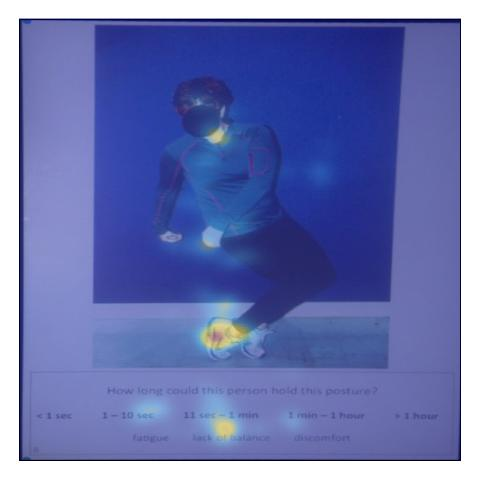
\includegraphics[width=0.49\textwidth]{figures/Kayd_heatmap_posture8.jpg} \hspace{1pt}
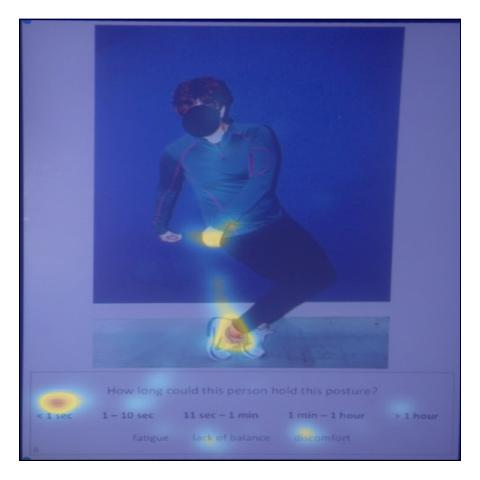
\includegraphics[width=0.49\textwidth]{figures/Subject13_heatmap_posture8.jpg} \\
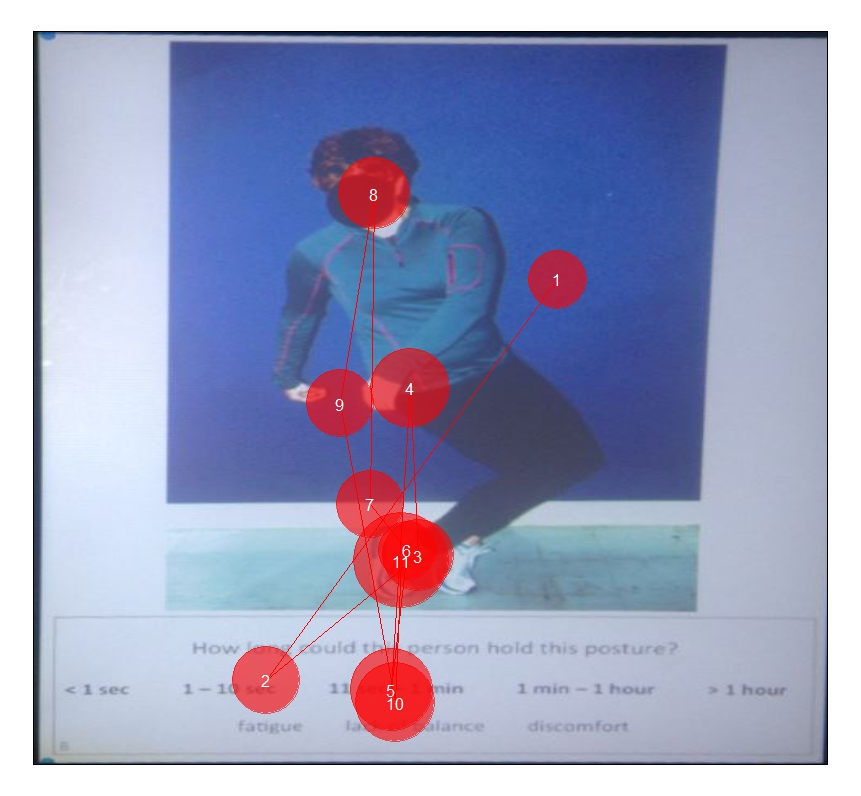
\includegraphics[width=0.49\textwidth]{figures/Kayd_scanpath_posture8.jpg} \hspace{1pt}
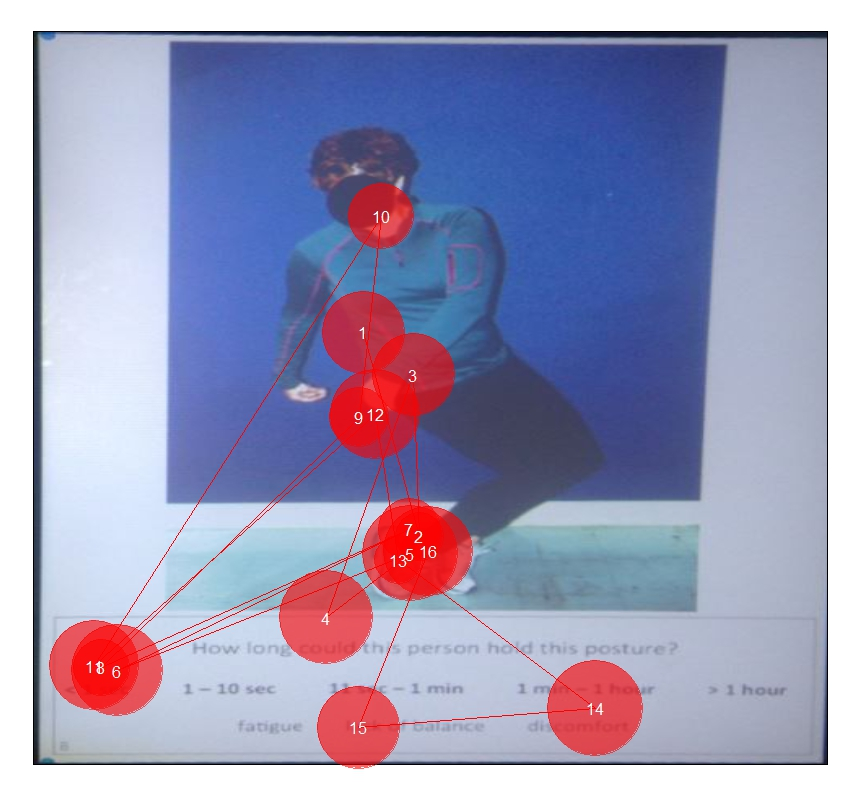
\includegraphics[width=0.49\textwidth]{figures/Subject13_scanpath_posture8.jpg}
\end{center}
\caption{\label{Posture8View}Posture 8: Different assessments (1sec--10sec vs $<$ 1sec),
but similar fixations (as shown in the attention maps in the top row) and 
similar saccades (as shown in the scanpaths in the bottom row)
for Participant~1 (left column) and Participant~2 (right column).
}
\end{figure}


For Posture~8, combination (v) occurred.
The two participants indicated that this posture could be kept for
1sec -- 10sec and $<$ 1sec, respectively. In fact, this was the only posture where
one of the two participants indicated that such a posture was highly unstable and
could only be kept for less than 1sec. While the assessments are different, the
fixations (see Figure~\ref{Posture8View}, top row) and also 
the saccades (see Figure~\ref{Posture8View}, bottom row) are similar.


%	\subsection{Posture 8: Scanpaths vs Linked Scanpath Microposter}
%	\begin{center} 
%		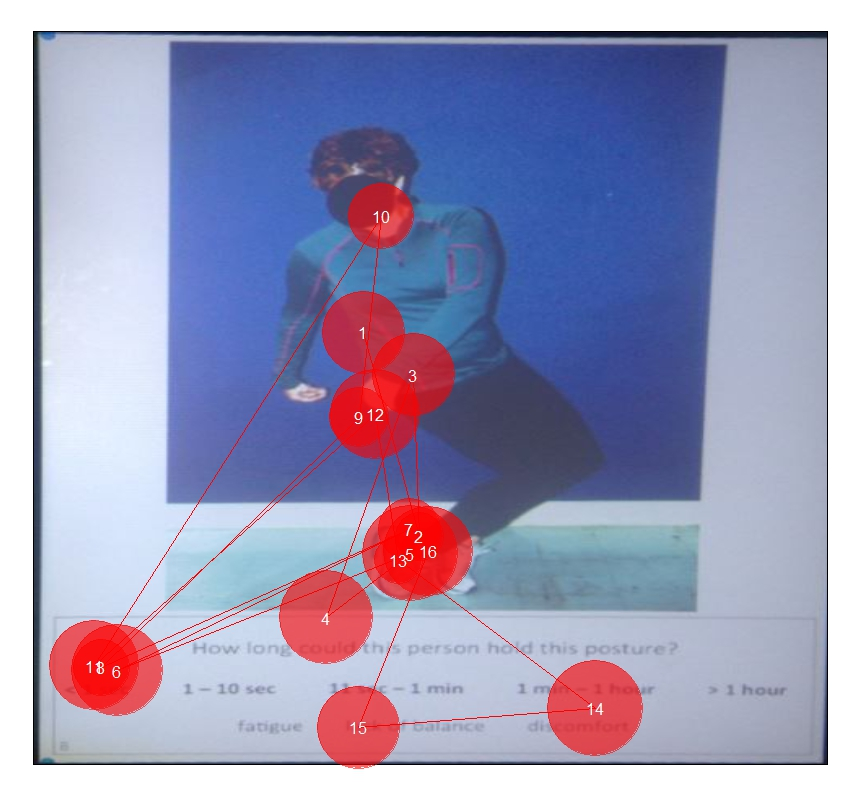
\includegraphics[width=5.5cm]{figures/Subject13_scanpath_posture8} \hspace{1pt}
%		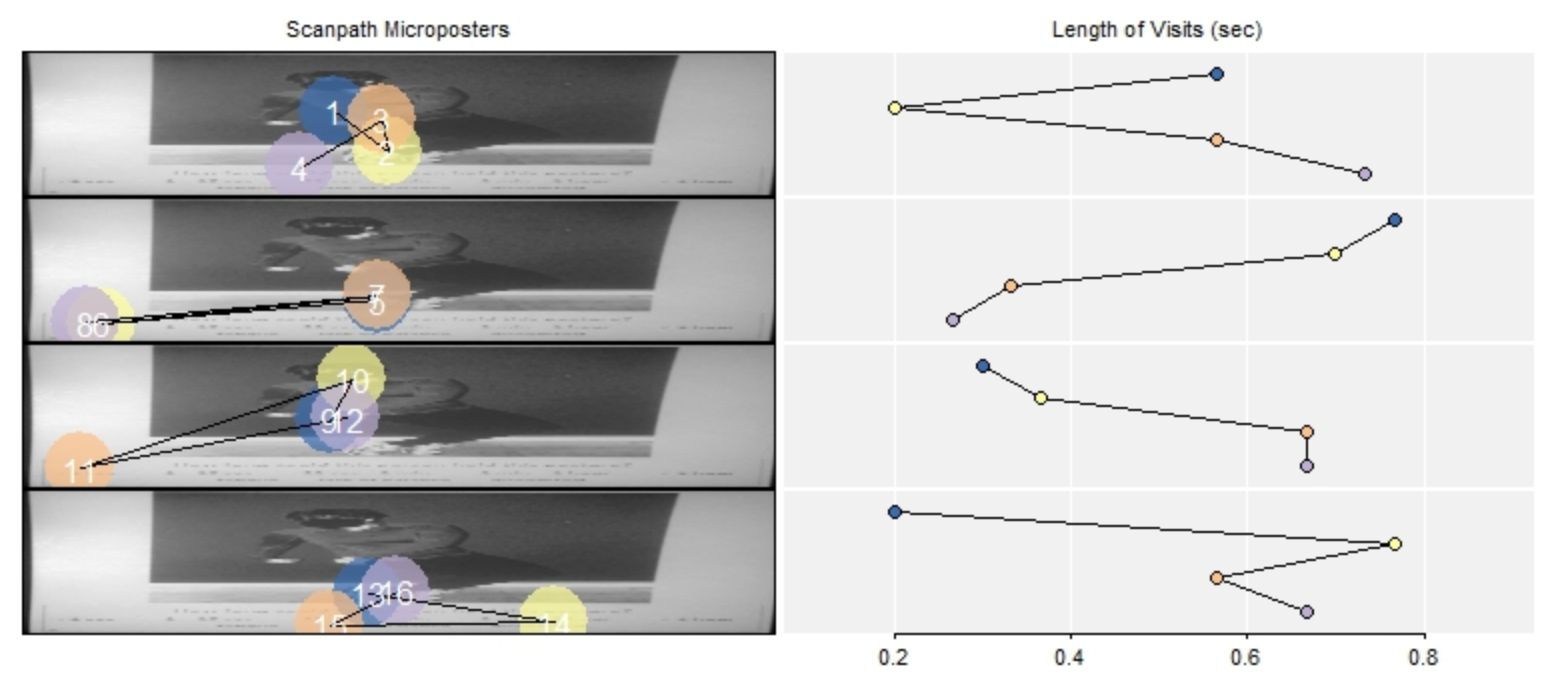
\includegraphics[height=5cm,width=4cm]{figures/Subject13_LSM_posture8_clipped.jpg}
%	\end{center}


\begin{figure}[t]
\begin{center} 
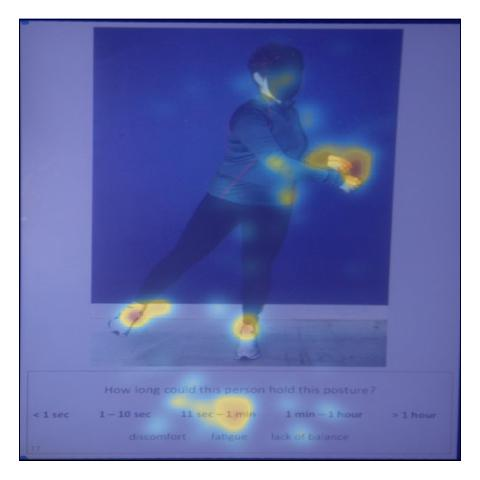
\includegraphics[width=0.49\textwidth]{figures/Kayd_heatmap_posture17.jpg} \hspace{1pt}
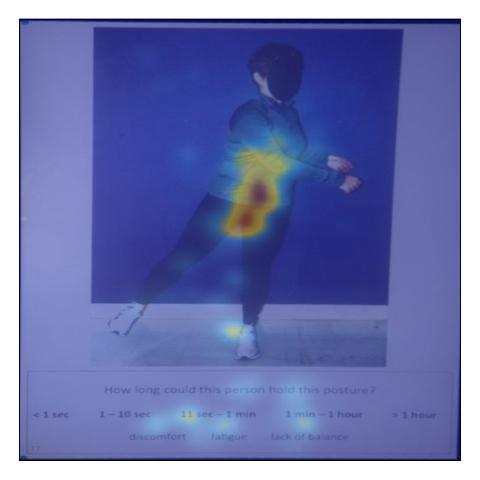
\includegraphics[width=0.49\textwidth]{figures/Subject13_heatmap_posture17.jpg}
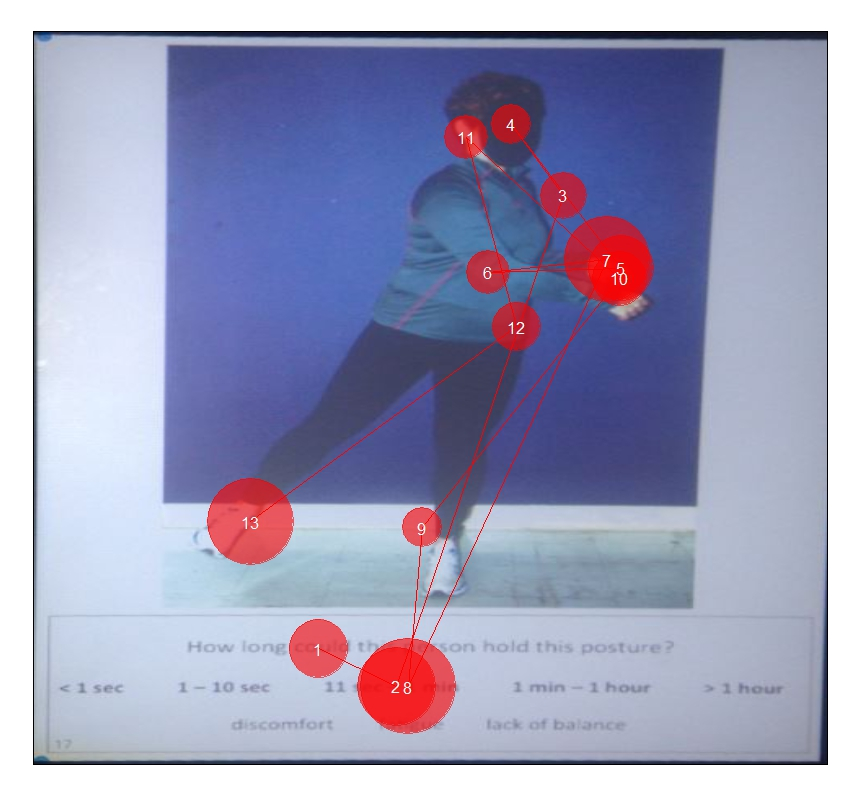
\includegraphics[width=0.49\textwidth]{figures/Kayd_scanpath_posture17.jpg} \hspace{1pt}
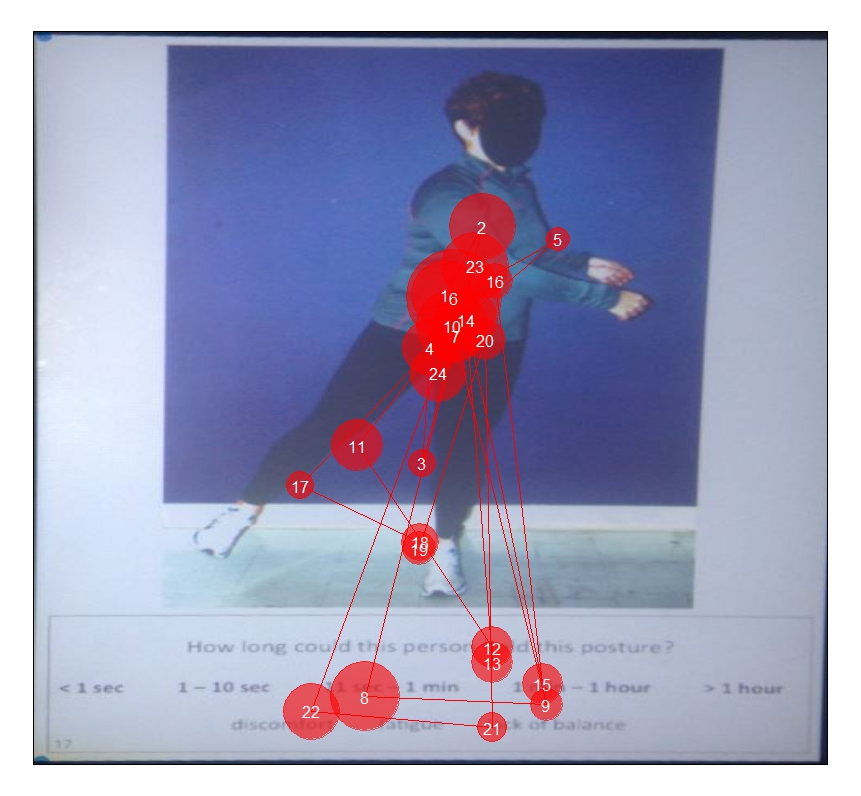
\includegraphics[width=0.49\textwidth]{figures/Subject13_scanpath_posture17.jpg}	
\end{center}
\caption{\label{Posture17View}Posture 17: Different assessments (11sec--1min vs 1min--1hour), 
and also different fixations (as shown in the attention maps in the top row) and 
different saccades (as shown in the scanpaths in the bottom row)
for Participant~1 (left column) and Participant~2 (right column).
}
\end{figure}


For Posture~17, combination (viii) occurred.
The two participants indicated that this posture could be kept for
11sec -- 1min and 1min -- 1hour, respectively. Moreover, the
fixations (see Figure~\ref{Posture17View}, top row) and also 
the saccades (see Figure~\ref{Posture17View}, bottom row) were different.


\begin{figure}[t]
\begin{center} 
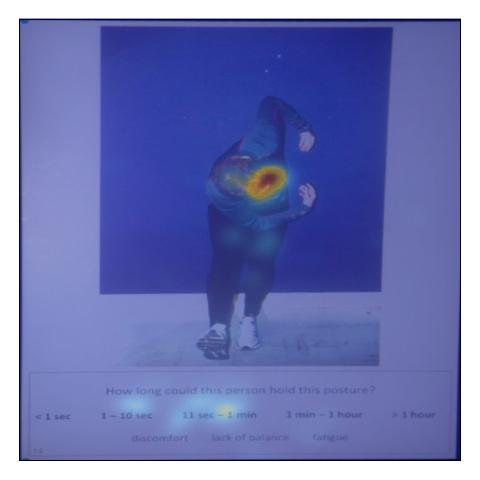
\includegraphics[width=0.49\textwidth]{figures/Kayd_heatmap_posture14.jpg} \hspace{1pt}
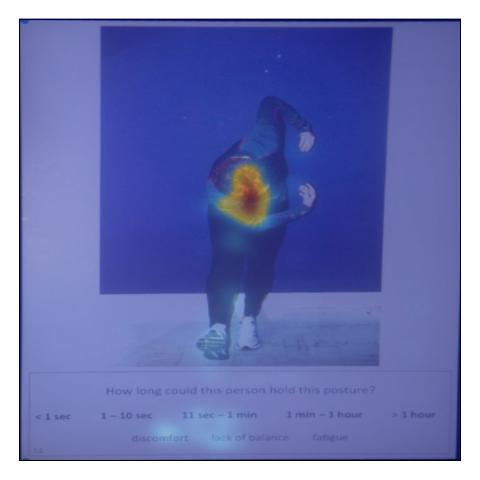
\includegraphics[width=0.49\textwidth]{figures/Subject13_heatmap_posture14.jpg}
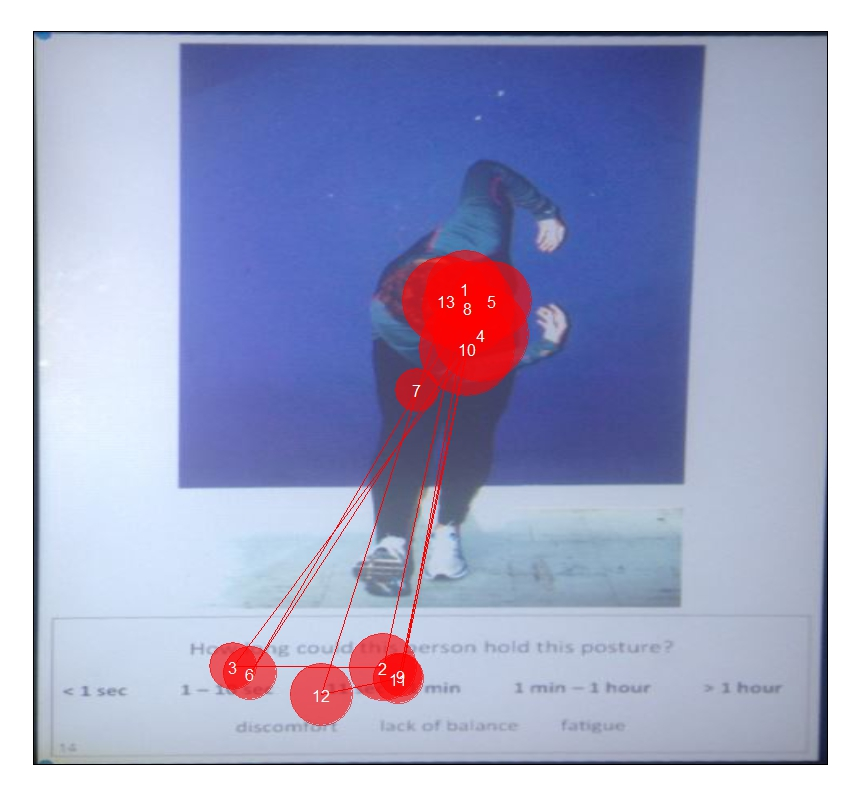
\includegraphics[width=0.49\textwidth]{figures/Kayd_scanpath_posture14.jpg} \hspace{1pt}
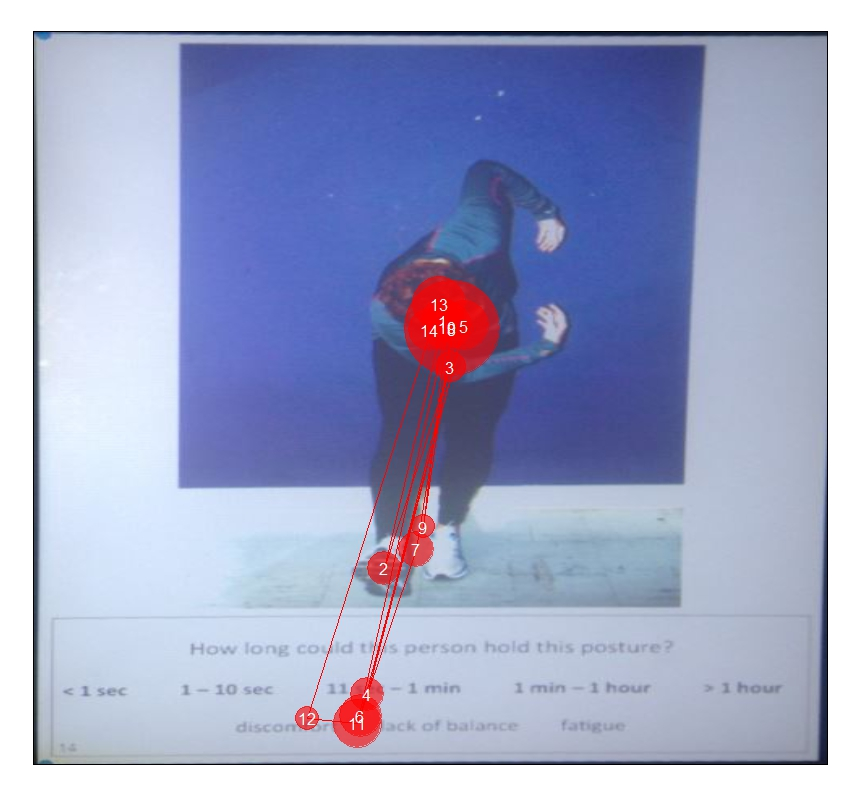
\includegraphics[width=0.49\textwidth]{figures/Subject13_scanpath_posture14.jpg}
\end{center}
\caption{\label{Posture14View}Posture 14: Identical assessments (11sec--1min both),
similar fixations (as shown in the attention maps in the top row) and 
similar saccades (as shown in the scanpaths in the bottom row)
for Participant~1 (left column) and Participant~2 (right column).
}
\end{figure}


For Posture~14, combination (i) occurred.
Both participants indicated that this posture could be kept for
11sec -- 1min. In addition to the assessments, the
fixations (see Figure~\ref{Posture14View}, top row) and also 
the saccades (see Figure~\ref{Posture14View}, bottom row) were similar.
However, one might as well argue that there are some additional fixations
from Participant~2, looking at the right foot of the actor in this posture.
These fixations and related saccades are only visible in the scanpath,
but not in the attention map. Some further work remains to be done to determine what constitutes
identical (or similar) fixations and scanpaths in the final study.


\subsection{Scanpath Maps vs Linked Scanpath Microposter Plots}
\label{ScanpathVsMicroposter}


\begin{figure}[t]
\begin{center} 
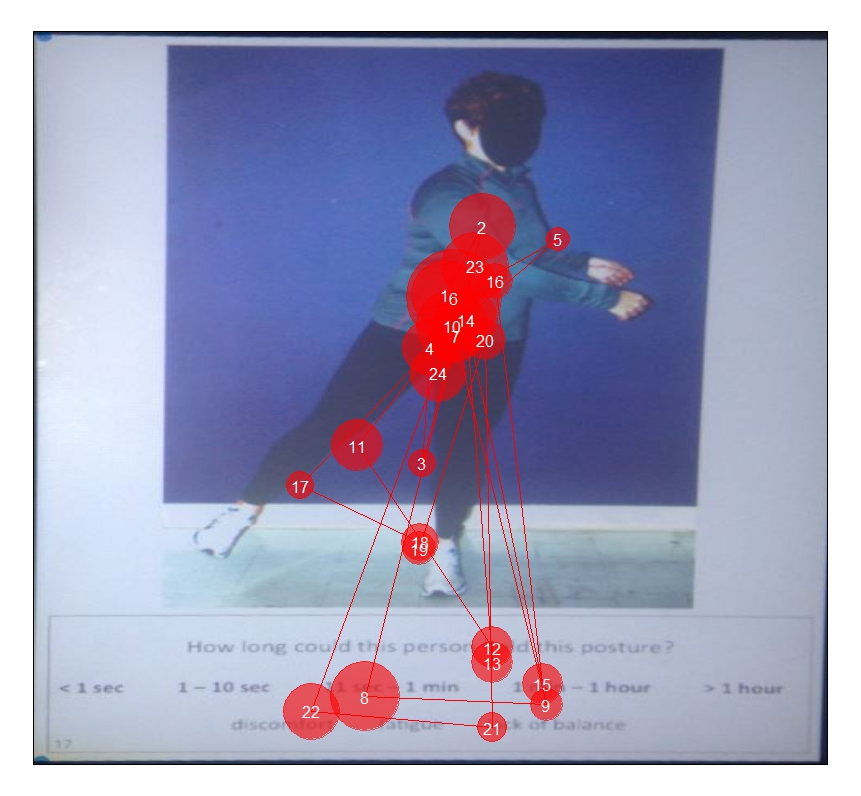
\includegraphics[width=0.49\textwidth]{figures/Subject13_scanpath_posture17.jpg} \hspace{1pt}
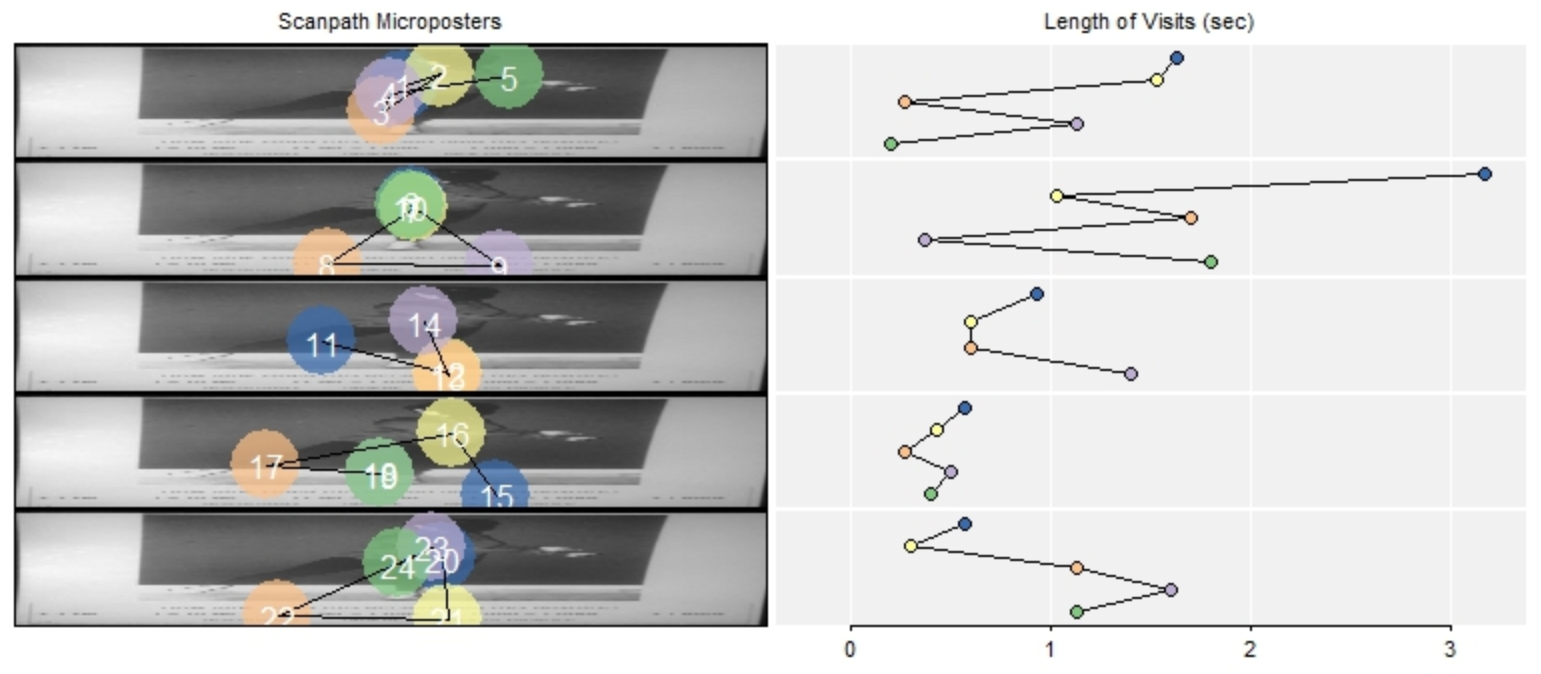
\includegraphics[height=0.45\textwidth,width=0.49\textwidth]{figures/Subject13_LSM_posture17_clipped.jpg}
\end{center}
\caption{\label{ScanpathsLSM17}Posture 17: Scanpath map (left) vs linked scanpath microposter plots (right) for Participant~2.}
\end{figure}


\begin{figure}[t]
\begin{center} 
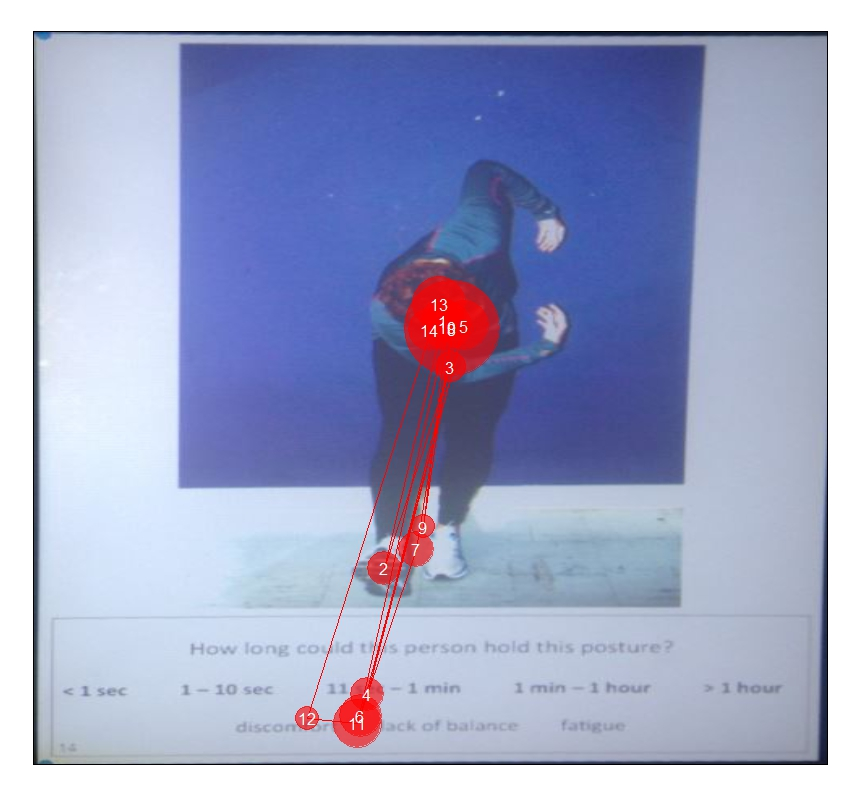
\includegraphics[width=0.49\textwidth]{figures/Subject13_scanpath_posture14.jpg} \hspace{1pt}
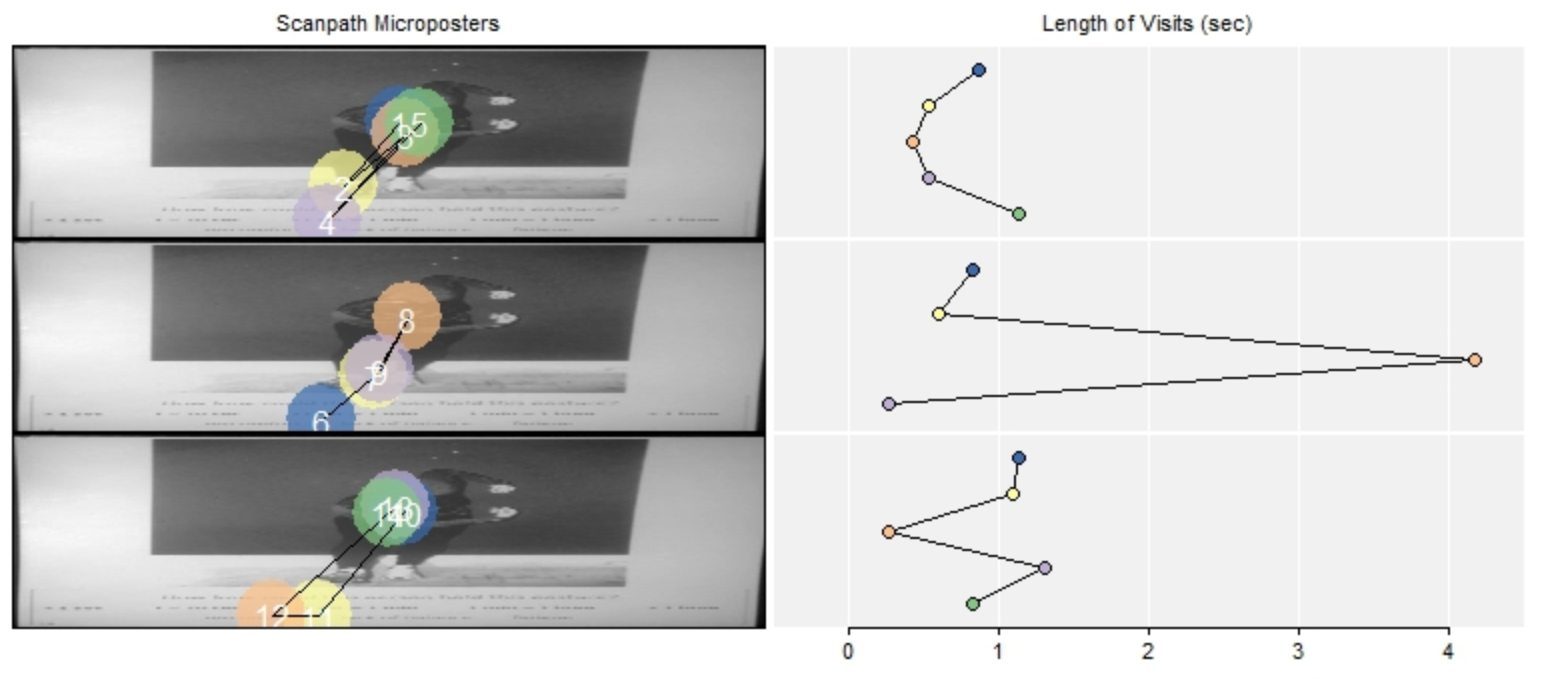
\includegraphics[height=0.45\textwidth,width=0.49\textwidth]{figures/Subject13_LSM_posture14_clipped.jpg}
\end{center}
\caption{\label{ScanpathsLSM14}Posture 14: Scanpath map (left) vs linked scanpath microposter plots (right) for Participant~2.}
\end{figure}


In addition to the traditional eye-tracking visualization methods presented so far, it is worthwhile to
apply some of the new visualization methods from \cite{LS2016ASA,LS2017ASA} to the postures used in this study.
These new visualization methods were originally developed for identifying important features of scientific posters.
In this section, we will contrast regular scanpaths with linked scanpath microposter plots
for Posture~17 (Figure~\ref{ScanpathsLSM17}) 
and Posture~14 (Figure~\ref{ScanpathsLSM14}), both for Participant~2. 
In a regular scanpath map, all fixations and saccades are overlaid on a single image, i.e., posture in this context.
This can often lead to extensive overplotting, making it difficult to identify the
labels, sizes, and exact locations of the fixations. 
In contrast, 
the fixations and saccades are broken down in several consecutive batches
of four to five fixations and saccades in linked scanpath microposter plots. 
Each of these batches is overlaid individually on an image
of the posture. Rather than using the size of circles to distinguish the lengths of the fixations as in scanpath maps,
linked scanpath microposter plots contain one (or more) statistical columns where statistical variables
can be shown. In this case, there is only one statistical column, showing dotplots for the lengths
of each fixation. While most fixations are relatively short (under 1sec), fixation 6 for Posture~17 lasts over 3sec
(Figure~\ref{ScanpathsLSM17}) and fixation 8 for Posture~14 lasts over 4sec
(Figure~\ref{ScanpathsLSM14}).



\subsection{The Problem of Detecting Meaningful Fixations}
\label{MeaningfulFixations}


Similar to detecting clusters in higher-dimensional data, detecting meaningful fixations highly depends
on the underlying method / algorithm selection and choices of the starting parameters.
In fact, fixations could be considered to be clusters in a 3--dimensional space--time coordinate system.
The {\tt EyeTrackR} R package makes use of the {\tt saccades} R package \citep{VDM2015}.
According to the description on its help page, the {\tt detect.fixations} function from this package
``takes a data frame containing raw eye-tracking samples and returns a data frame containing fixations.''
An input argument for this function, called {\it lambda}, is defined as follows:
``a parameter for tuning the saccade detection. It specifies which multiple of the standard deviation of the velocity 
distribution should be used as the detection threshold.''
It turns out that different choices for {\it lambda} result in rather large variations in the number
of fixations that are detected, and also in the actual locations of these fixations, as outlined
in the following three examples.

The  {\tt detect.fixations} function from the {\tt saccades} R package
uses a velocity-based fixation detection algorithm for saccades, introduced by \cite{EK2003}.
\cite{SG2000} provided a taxonomy of fixation identification algorithms and conducted
a qualitative assessment of five different algorithms. They came to the conclusion that
``the choice of identification algorithms can dramatically
affect the resulting identified fixations.''


\begin{figure}[t]
\begin{center} 
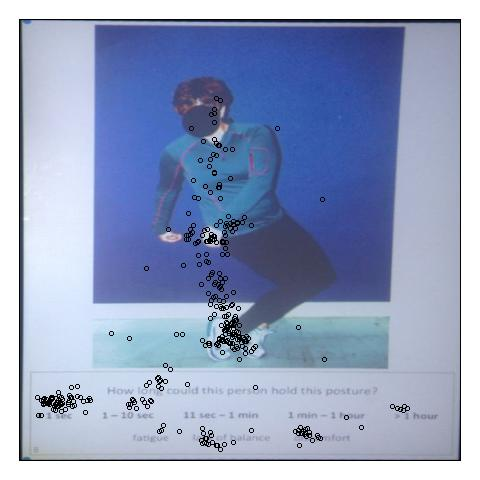
\includegraphics[width=0.30\textwidth]{figures/Subject13_scatterplot_posture8.jpg} \hspace{1pt}
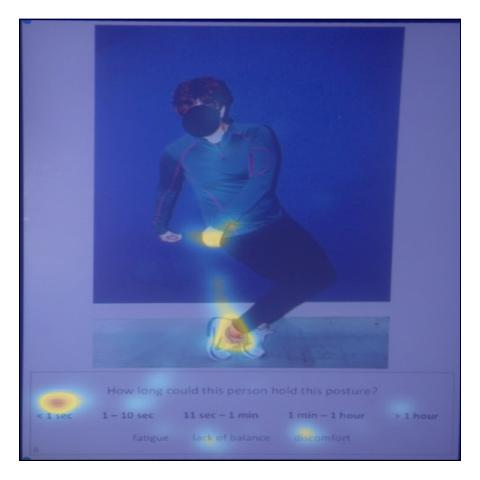
\includegraphics[width=0.30\textwidth]{figures/Subject13_heatmap_posture8_new.jpg} \\
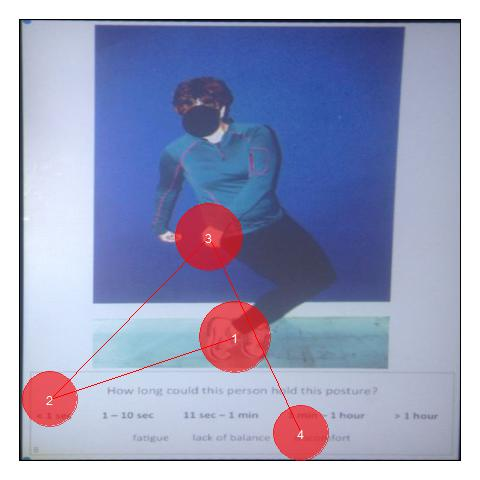
\includegraphics[width=0.30\textwidth]{figures/Subject13_scanpath_posture8_lambda_1.jpg} \hspace{1pt}
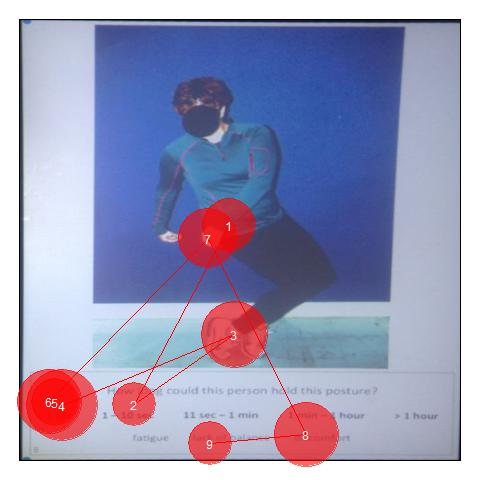
\includegraphics[width=0.30\textwidth]{figures/Subject13_scanpath_posture8_lambda_2.jpg} \\
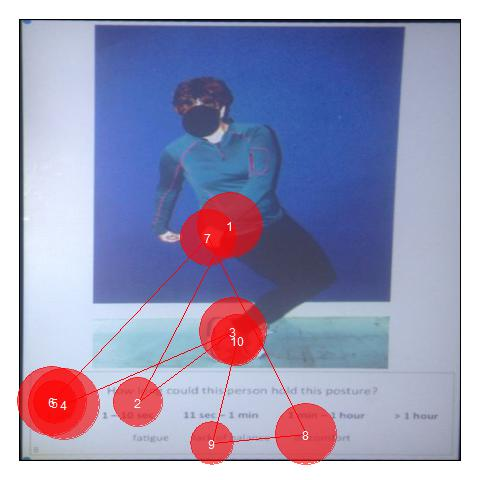
\includegraphics[width=0.30\textwidth]{figures/Subject13_scanpath_posture8_lambda_3.jpg} \hspace{1pt}
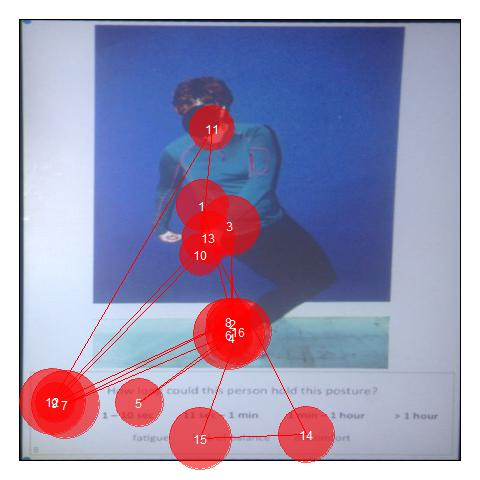
\includegraphics[width=0.30\textwidth]{figures/Subject13_scanpath_posture8_lambda_5.jpg} \\
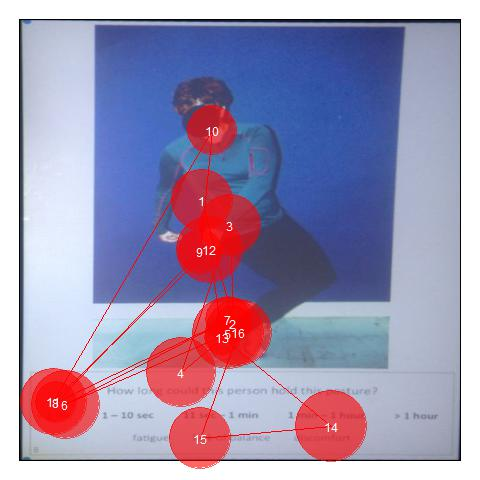
\includegraphics[width=0.30\textwidth]{figures/Subject13_scanpath_posture8_lambda_8.jpg} \hspace{1pt}
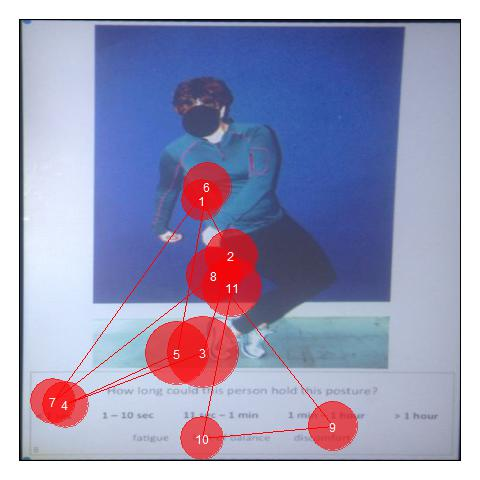
\includegraphics[width=0.30\textwidth]{figures/Subject13_scanpath_posture8_lambda_10.jpg} \\
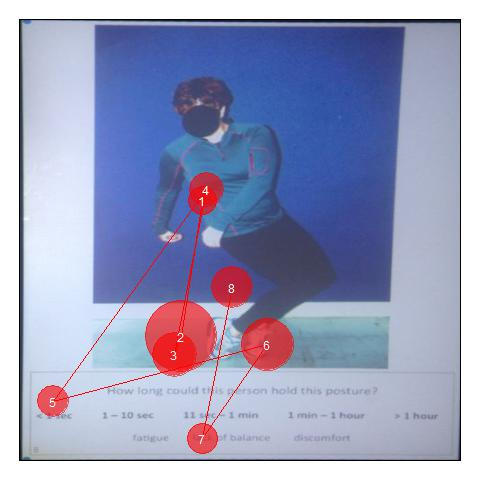
\includegraphics[width=0.30\textwidth]{figures/Subject13_scanpath_posture8_lambda_12.jpg} \hspace{1pt}
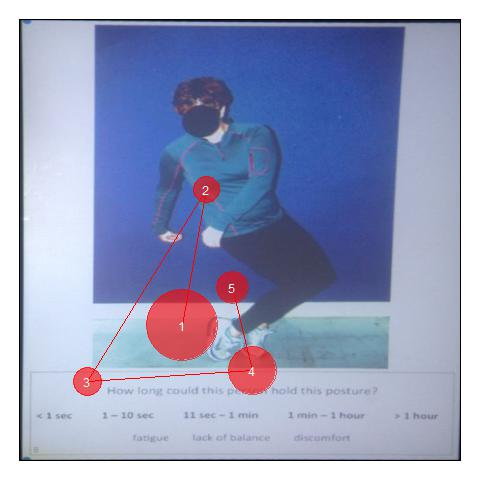
\includegraphics[width=0.30\textwidth]{figures/Subject13_scanpath_posture8_lambda_15.jpg}
\end{center} ~\\[-1.5cm]
\caption{\label{Fixations8}Posture 8: Different fixations detected for Participant~2, based on different values
for {\it lambda} (1, 2, 3, 5, 8, 10, 12, 15 row-wise from top left to bottom right). For comparison,
a scatterplot and attention map of the underlying focus points are shown in the top row.}
\end{figure}


Figure~\ref{Fixations8} shows the fixations and saccades for eight different values of {\it lambda} for
Posture~8 for Participant~2. The number of fixations detected increased from 4 (for {\it lambda} $=$ 1)
to 16 (for {\it lambda} $=$ 8) and then decreased again to 5 (for {\it lambda} $=$ 15). 
A likely fixation at the chin/head area only was detected for {\it lambda} $=$ 5 and 8,
making these the best choices here.
Small values of {\it lambda} missed most of the fixations in the text area at the bottom.
Large values of {\it lambda} combined several fixations into a single artificial fixation
at the spatial center of the combined fixations. This becomes most obvious
for {\it lambda} $=$ 12 and 15 where no fixation is located at the left hand of the actor.

Figure~\ref{Fixations17} shows the fixations and saccades for eight different values of {\it lambda} for
Posture~17 for Participant~2. The number of fixations detected increased from 8 (for {\it lambda} $=$ 1)
to 30 (for {\it lambda} $=$ 5) and then decreased again to 11 (for {\it lambda} $=$ 15). 
The smallest value of {\it lambda} missed most of the fixations in the text area at the bottom.
Again, large values of {\it lambda} combined several fixations. This becomes most obvious
for {\it lambda} $=$ 10, 12, and 15 where no fixation is located in the lower left of the text area.
The best choices again are {\it lambda} $=$ 5 and 8.

Figure~\ref{Fixations14} shows the fixations and saccades for eight different values of {\it lambda} for
Posture~14 for Participant~2. The number of fixations detected increased from 6 (for {\it lambda} $=$ 1)
to 19 (for {\it lambda} $=$ 5) and then decreased again to 11 (for {\it lambda} $=$ 15). 
Small values of {\it lambda} missed most of the fixations in the text area at the bottom.
Once more, large values of {\it lambda} combined several fixations. This becomes most obvious
for {\it lambda} $=$ 15 where an additional fixation is located in the upper leg area of the actor.
The best choices once more are {\it lambda} $=$ 5 and 8.

Based on the observations from Figures~\ref{Fixations8} to \ref{Fixations14},
{\it lambda} $=$ 8 has been selected for both participants
for the scanpath maps and linked scanpath microposter plots from Figures~\ref{Posture8View} to \ref{ScanpathsLSM14}.
While this is a reasonable
choice here, this needs some careful reassessment in the full study.


\begin{figure}[t]
\begin{center} 
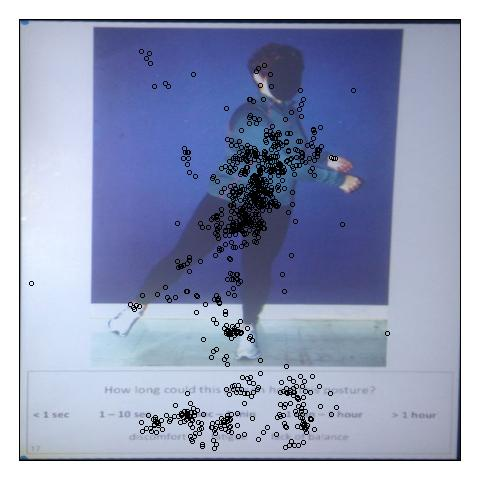
\includegraphics[width=0.30\textwidth]{figures/Subject13_scatterplot_posture17.jpg} \hspace{1pt}
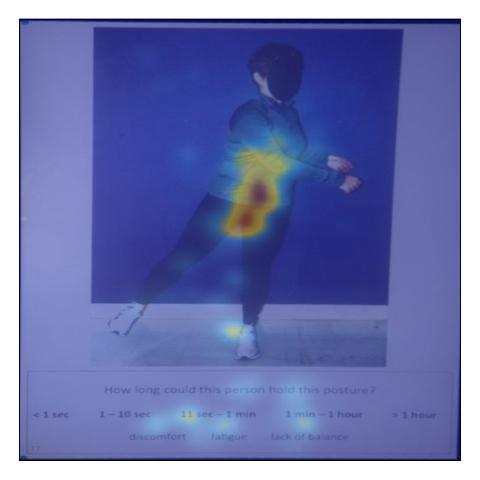
\includegraphics[width=0.30\textwidth]{figures/Subject13_heatmap_posture17_new.jpg} \\
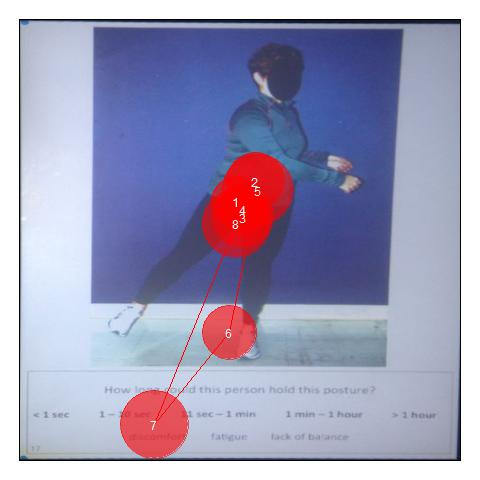
\includegraphics[width=0.30\textwidth]{figures/Subject13_scanpath_posture17_lambda_1.jpg} \hspace{1pt}
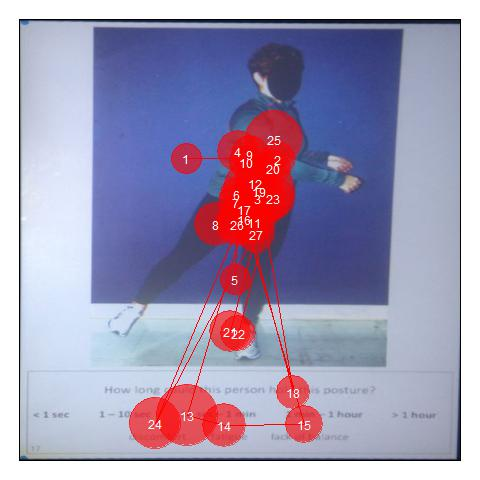
\includegraphics[width=0.30\textwidth]{figures/Subject13_scanpath_posture17_lambda_2.jpg} \\
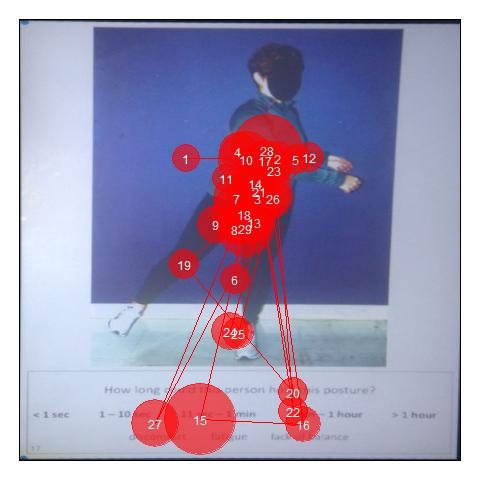
\includegraphics[width=0.30\textwidth]{figures/Subject13_scanpath_posture17_lambda_3.jpg} \hspace{1pt}
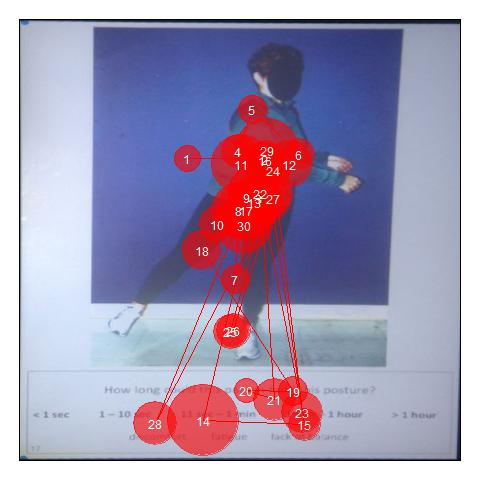
\includegraphics[width=0.30\textwidth]{figures/Subject13_scanpath_posture17_lambda_5.jpg} \\
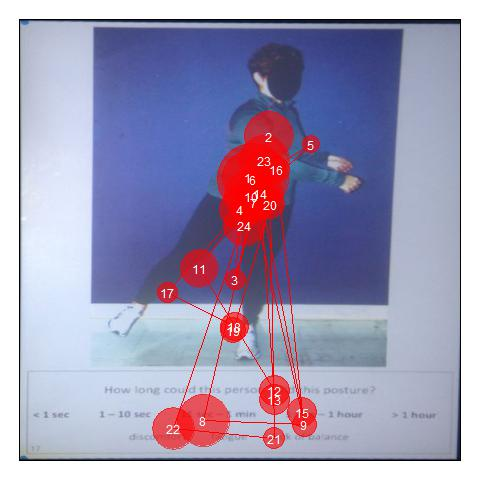
\includegraphics[width=0.30\textwidth]{figures/Subject13_scanpath_posture17_lambda_8.jpg} \hspace{1pt}
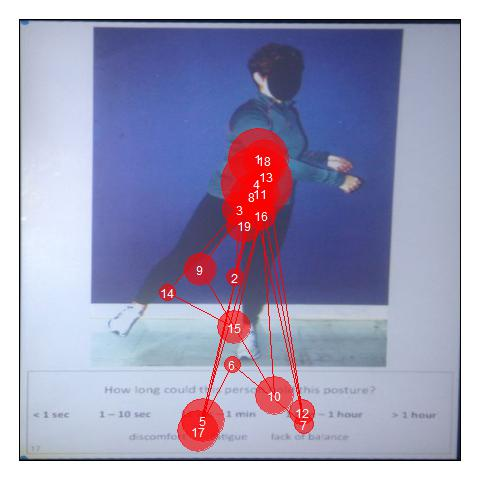
\includegraphics[width=0.30\textwidth]{figures/Subject13_scanpath_posture17_lambda_10.jpg} \\
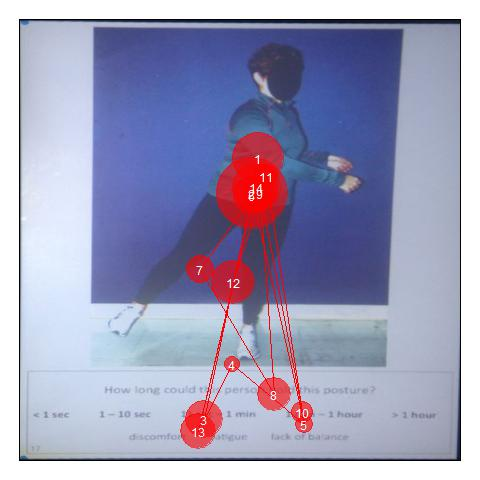
\includegraphics[width=0.30\textwidth]{figures/Subject13_scanpath_posture17_lambda_12.jpg} \hspace{1pt}
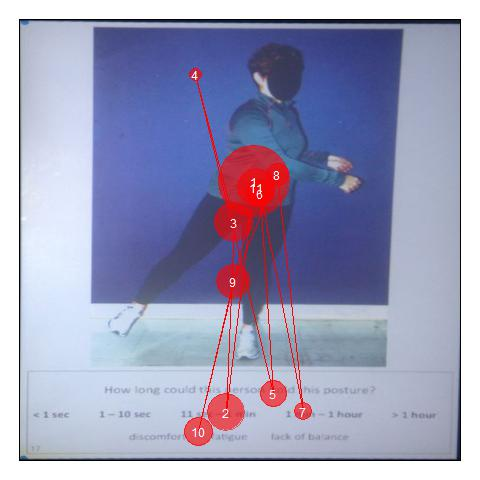
\includegraphics[width=0.30\textwidth]{figures/Subject13_scanpath_posture17_lambda_15.jpg}
\end{center} ~\\[-1.5cm]
\caption{\label{Fixations17}Posture 17: Different fixations detected for Participant~2, based on different values
for {\it lambda} (1, 2, 3, 5, 8, 10, 12, 15 row-wise from top left to bottom right). For comparison,
a scatterplot and attention map of the underlying focus points are shown in the top row.}
\end{figure}


\begin{figure}[t]
\begin{center} 
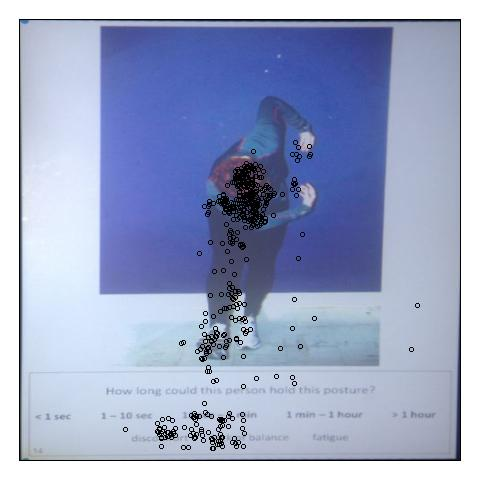
\includegraphics[width=0.30\textwidth]{figures/Subject13_scatterplot_posture14.jpg} \hspace{1pt}
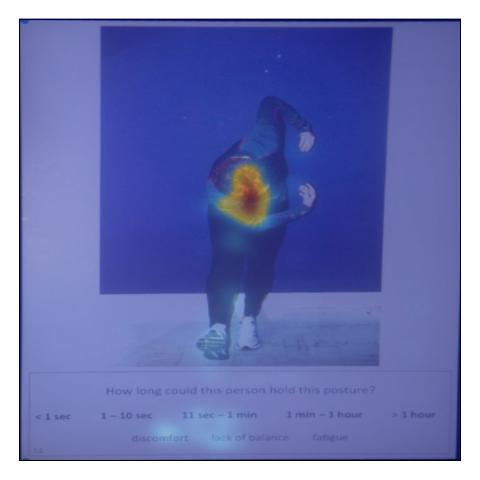
\includegraphics[width=0.30\textwidth]{figures/Subject13_heatmap_posture14_new.jpg} \\
\includegraphics[width=0.30\textwidth]{figures/Subject13_scanpath_posture14_lambda_1.jpg} \hspace{1pt}
\includegraphics[width=0.30\textwidth]{figures/Subject13_scanpath_posture14_lambda_2.jpg} \\
\includegraphics[width=0.30\textwidth]{figures/Subject13_scanpath_posture14_lambda_3.jpg} \hspace{1pt}
\includegraphics[width=0.30\textwidth]{figures/Subject13_scanpath_posture14_lambda_5.jpg} \\
\includegraphics[width=0.30\textwidth]{figures/Subject13_scanpath_posture14_lambda_8.jpg} \hspace{1pt}
\includegraphics[width=0.30\textwidth]{figures/Subject13_scanpath_posture14_lambda_10.jpg} \\
\includegraphics[width=0.30\textwidth]{figures/Subject13_scanpath_posture14_lambda_12.jpg} \hspace{1pt}
\includegraphics[width=0.30\textwidth]{figures/Subject13_scanpath_posture14_lambda_15.jpg}
\end{center} ~\\[-1.5cm]
\caption{\label{Fixations14}Posture 14: Different fixations detected for Participant~2, based on different values
for {\it lambda} (1, 2, 3, 5, 8, 10, 12, 15 row-wise from top left to bottom right). For comparison,
a scatterplot and attention map of the underlying focus points are shown in the top row.}
\end{figure}


%%%%%%%%%%%%%%%%%%%%%%%%%
\section{Outlook on Main Study}  
\label{Outlook}
%%%%%%%%%%%%%%%%%%%%%%%%%


The preliminary results for the two test participants presented in this article were obtained after
numerous small changes and modifications over the course of several months.
Some of the questions we had to answer were how to present the postures,
e.g., as printouts or projected on a wall. How far should the participants be located
away from the printout/projection? Should the participants stand or be seated ---
and should they be allowed to freely move around? 
Other questions were related to the actual presentation of the postures, e.g., what kind
of background or frame should be used around the actual images of the postures and
how to separate consecutive postures so that there is no overlap of the eye position
from a previous posture when the next posture is shown. Ultimately,
after deciding on projecting the postures on a white wall, questions arose which
computer and projector to use and how to adjust the lighting in the room
(as different computers and projectors have different light intensities and resolutions).

Ultimately, the results from the two participants presented here were obtained from
the final setup,  except one remaining modification: The text area of the postures
still shows a possible reason why a posture has to be given up (with options
``fatigue,'' ``lack of balance,'' and ``discomfort''). These options will no
longer be shown in the full study and the participants won't be asked any
related questions.

The eye-tracking technology provided satisfactory and detailed information about which body parts the participants looked at
that hopefully will allow us to draw further quantitative conclusions beyond EDA in the full study.
Nevertheless, EDA will remain an important component for the analysis of the data from the full study,
in particular to confirm the proper calibration of the eye-tracking device (as seen in Figure~\ref{ScatterplotPrePost}) and
to assess how meaningful automatically identified fixations are (as discussed in Section~\ref{MeaningfulFixations}).
Scatterplots, attention maps, scanpath maps, linked scanpath microposter plots, and other visualization methods will 
be effective means to summarize and communicate the data and results from the participants in the full study.

At this time, we believe we are ready to start with the data collection for the full study
in the 2017/2018 academic year. The necessary approval from the Institutional Review Board (IRB)
at USU has been obtained and fliers that advertise the participation in this study are
ready to be posted in buildings and electronically. We are eager to obtain, analyze, and
present the data and results from the full posture study, given the promising
exploratory results from these two test participants.


\bibliographystyle{elsarticle-harv}
% modified to add 
%     \itemsep=0pt
% to 2nd line of file paper.bbl

\bibliography{references}


\end{document}

